% Options for packages loaded elsewhere
% Options for packages loaded elsewhere
\PassOptionsToPackage{unicode}{hyperref}
\PassOptionsToPackage{hyphens}{url}
\PassOptionsToPackage{dvipsnames,svgnames,x11names}{xcolor}
%
\documentclass[
  letterpaper,
  DIV=11,
  numbers=noendperiod]{scrartcl}
\usepackage{xcolor}
\usepackage[margin=0.75in]{geometry}
\usepackage{amsmath,amssymb}
\setcounter{secnumdepth}{-\maxdimen} % remove section numbering
\usepackage{iftex}
\ifPDFTeX
  \usepackage[T1]{fontenc}
  \usepackage[utf8]{inputenc}
  \usepackage{textcomp} % provide euro and other symbols
\else % if luatex or xetex
  \usepackage{unicode-math} % this also loads fontspec
  \defaultfontfeatures{Scale=MatchLowercase}
  \defaultfontfeatures[\rmfamily]{Ligatures=TeX,Scale=1}
\fi
\usepackage{lmodern}
\ifPDFTeX\else
  % xetex/luatex font selection
\fi
% Use upquote if available, for straight quotes in verbatim environments
\IfFileExists{upquote.sty}{\usepackage{upquote}}{}
\IfFileExists{microtype.sty}{% use microtype if available
  \usepackage[]{microtype}
  \UseMicrotypeSet[protrusion]{basicmath} % disable protrusion for tt fonts
}{}
\makeatletter
\@ifundefined{KOMAClassName}{% if non-KOMA class
  \IfFileExists{parskip.sty}{%
    \usepackage{parskip}
  }{% else
    \setlength{\parindent}{0pt}
    \setlength{\parskip}{6pt plus 2pt minus 1pt}}
}{% if KOMA class
  \KOMAoptions{parskip=half}}
\makeatother
% Make \paragraph and \subparagraph free-standing
\makeatletter
\ifx\paragraph\undefined\else
  \let\oldparagraph\paragraph
  \renewcommand{\paragraph}{
    \@ifstar
      \xxxParagraphStar
      \xxxParagraphNoStar
  }
  \newcommand{\xxxParagraphStar}[1]{\oldparagraph*{#1}\mbox{}}
  \newcommand{\xxxParagraphNoStar}[1]{\oldparagraph{#1}\mbox{}}
\fi
\ifx\subparagraph\undefined\else
  \let\oldsubparagraph\subparagraph
  \renewcommand{\subparagraph}{
    \@ifstar
      \xxxSubParagraphStar
      \xxxSubParagraphNoStar
  }
  \newcommand{\xxxSubParagraphStar}[1]{\oldsubparagraph*{#1}\mbox{}}
  \newcommand{\xxxSubParagraphNoStar}[1]{\oldsubparagraph{#1}\mbox{}}
\fi
\makeatother


\usepackage{longtable,booktabs,array}
\newcounter{none} % for unnumbered tables
\usepackage{calc} % for calculating minipage widths
% Correct order of tables after \paragraph or \subparagraph
\usepackage{etoolbox}
\makeatletter
\patchcmd\longtable{\par}{\if@noskipsec\mbox{}\fi\par}{}{}
\makeatother
% Allow footnotes in longtable head/foot
\IfFileExists{footnotehyper.sty}{\usepackage{footnotehyper}}{\usepackage{footnote}}
\makesavenoteenv{longtable}
\usepackage{graphicx}
\makeatletter
\newsavebox\pandoc@box
\newcommand*\pandocbounded[1]{% scales image to fit in text height/width
  \sbox\pandoc@box{#1}%
  \Gscale@div\@tempa{\textheight}{\dimexpr\ht\pandoc@box+\dp\pandoc@box\relax}%
  \Gscale@div\@tempb{\linewidth}{\wd\pandoc@box}%
  \ifdim\@tempb\p@<\@tempa\p@\let\@tempa\@tempb\fi% select the smaller of both
  \ifdim\@tempa\p@<\p@\scalebox{\@tempa}{\usebox\pandoc@box}%
  \else\usebox{\pandoc@box}%
  \fi%
}
% Set default figure placement to htbp
\def\fps@figure{htbp}
\makeatother





\setlength{\emergencystretch}{3em} % prevent overfull lines

\providecommand{\tightlist}{%
  \setlength{\itemsep}{0pt}\setlength{\parskip}{0pt}}



 


\usepackage{booktabs}
\usepackage{longtable}
\usepackage{array}
\usepackage{multirow}
\usepackage{wrapfig}
\usepackage{float}
\usepackage{colortbl}
\usepackage{pdflscape}
\usepackage{tabu}
\usepackage{threeparttable}
\usepackage{threeparttablex}
\usepackage[normalem]{ulem}
\usepackage{makecell}
\usepackage{xcolor}
\usepackage{caption}
\usepackage{anyfontsize}
\KOMAoption{captions}{tableheading}
\makeatletter
\@ifpackageloaded{caption}{}{\usepackage{caption}}
\AtBeginDocument{%
\ifdefined\contentsname
  \renewcommand*\contentsname{Table of contents}
\else
  \newcommand\contentsname{Table of contents}
\fi
\ifdefined\listfigurename
  \renewcommand*\listfigurename{List of Figures}
\else
  \newcommand\listfigurename{List of Figures}
\fi
\ifdefined\listtablename
  \renewcommand*\listtablename{List of Tables}
\else
  \newcommand\listtablename{List of Tables}
\fi
\ifdefined\figurename
  \renewcommand*\figurename{Figure}
\else
  \newcommand\figurename{Figure}
\fi
\ifdefined\tablename
  \renewcommand*\tablename{Table}
\else
  \newcommand\tablename{Table}
\fi
}
\@ifpackageloaded{float}{}{\usepackage{float}}
\floatstyle{ruled}
\@ifundefined{c@chapter}{\newfloat{codelisting}{h}{lop}}{\newfloat{codelisting}{h}{lop}[chapter]}
\floatname{codelisting}{Listing}
\newcommand*\listoflistings{\listof{codelisting}{List of Listings}}
\makeatother
\makeatletter
\makeatother
\makeatletter
\@ifpackageloaded{caption}{}{\usepackage{caption}}
\@ifpackageloaded{subcaption}{}{\usepackage{subcaption}}
\makeatother
\usepackage{bookmark}
\IfFileExists{xurl.sty}{\usepackage{xurl}}{} % add URL line breaks if available
\urlstyle{same}
\hypersetup{
  pdftitle={A cross-sectional observational study on the impact of cost on cardiac events in adults using simulated data},
  colorlinks=true,
  linkcolor={blue},
  filecolor={Maroon},
  citecolor={Blue},
  urlcolor={Blue},
  pdfcreator={LaTeX via pandoc}}


\title{A cross-sectional observational study on the impact of cost on
cardiac events in adults using simulated data}
\author{Tracy Chidyausiku}
\date{}
\begin{document}
\maketitle


\subsection{Introduction}\label{introduction}

In the United States, the overwhelming majority of adults experiencing
cardiac events fall disproportionately on individuals experiencing
poverty (low to very low income) on the county and federal levels.
Cardiac events are closely linked with ongoing cardiovascular diseases
in patients and are the leading cause of death in the United States. As
a result, rates in cardiovascular disease and death in low to very low
income individuals have increased at an alarming rate in recent years
and are only expected to more than triple in the next five years. To
better understand the social mechanisms, primarily financial factors
like medical costs, that impact an individual's ability to prevent or
delay cardiac events we used synthetic data to measure how cost
influences cardiac events.

The study objective is to measure how cost of care influences cardiac
events in the presence of controlling for biological and social factors
including age, sex, and smoking. We hypothesize that higher medical
costs are associated with an increase in cardiac events when controlling
for age, sex, and smoking.

\subsection{Methods}\label{methods}

A cross-sectional study using synthetic data from the Department of
Health Policy at Stanford University was conducted to investigate how
medical costs impact cardiac events in adult patients.

\subsubsection{Dataset}\label{dataset}

Data was used from a synthetic data set created by the Health Policy
Department at Stanford University (Sherri Rose, PhD). The data are
synthetic and developed in 2026 trained using de-identified health data
from a national dataset of adult (18 years and older) cardiac
hospitalizations in the United States from 2025. The synthetic dataset
is publicly accessible
(\url{https://github.com/MethodsForReproducibleHealthResearch/Assignment2}).
The dataset contains 5,000 synthetic adult health records with variables
including medical costs, cardiac events, sex, age, and smoking status.

\subsubsection{Study Population}\label{study-population}

The synthetic data consists of a 5,000 observations with no missing
data. The dataset was evaluated in its entirety, with no exclusions
based on outliers or key variables for a complete-case analysis. The
final analysis included all 5,000 observations originally developed
synthetically in the dataset.

\subsubsection{Study Variables and
Outcome}\label{study-variables-and-outcome}

Cardiac events may include any sudden, serious problem impacting the
cardiovascular system, particularly the heart. All synthetic data were
developed based on the data collection and observations in a national
dataset of adult (18 years and older) cardiac hospitalizations in the
United States from 2025. Based on the national dataset, cardiac events
were pre-defined and measured in the dataset as a binary variable (e.g.,
yes or no if a cardiac event was observed in the patient) based on ICD-9
and ICD-10 codes coded by the care team or hospital. In this study, the
dependent variable was cardiac events and was measured using the
synthetic dataset's pre-defined and measured reports as stated above.
The primary independent variable in this study was medical costs. Based
on the national dataset, medical costs were collected and measured in
the dataset for each observation. Medical costs were calculated by the
hospital billing team based on the type of care received given the
particular cardiac event experienced by the patient at the point-of-care
and time received. Potential confounders include sex, age, and gender.
All potential confounders were self-reported by patients for hospital
system record collections and are routinely collected during admission
to hospital stays or to receive care.

Biological and behavioral health factors (sex, age, smoking) were
selected a priori based on prior research and established causal
diagrams in literature showing the association and influence of these
factors on financial factors and cardiac events. All study variables
were assessed in their original, individual item level. No variables
were combined into composite indices, nor were any continuous variables
transformed into categorical groupings. We assessed biases such as
selection bias in the dependent, independent, and potential confounders
using Pearson's Chi-squared test and Wilcoxon rank sum test and visually
assessed spread of potential confounders using histograms.

\subsubsection{Statistical Analysis}\label{statistical-analysis}

We used logistic regression (using R's \emph{stats} built-in package) to
evaluate the odds ratios and 95\% confidence intervals (CI) for the
relationship between medical costs and cardiac events controlling for
sex, age, and smoking. Reference groups for categorical variables sex
and smoking include male and non-smoker, respectively. Logistic
regression is a classification algorithm that models the log-odds of an
event occurring by optimizing coefficients using maximum likelihood
estimation. The logistic regression hypothesis is modeled by predictors
\(x\) and coefficients \(\theta\):
\[h_{\theta} = \frac{1}{1 + e^{-\theta^Tx}}\]

For this study, our logistic regression equation was modeled with
cardiac event (yes or no) as the dependent variable and medical cost as
the primary independent variable. To control for confounding, our model
also adjusted for sex, age, and smoking. Specifically, let \(Y\)
represent a given outcome for an individual \(i\):

\[Y_i = \alpha + \beta_1Cost_{1,i} + \beta_2Sex_{2,i} + \beta_3Smoke_{3,i} + \beta_4Age_{4,i}\]

\(Cost\) is the indicator for medical cost related to the observed
cardiac event, \(Sex\) is an indicator for the self-reported sex (male
or female) by the individual, \(Smoke\) is the indicator for the
self-reported smoking status of the patient when the data were
collected, and \(Age\) is the self-reported age of the patient. Each
indicator is calculated for every individual \(i\) in the dataset. All
analyses were performed in RStudio (Version 2026.04.0+526).

\subsection{Results}\label{results}

\subsubsection{Population Demographics}\label{population-demographics}

Among the 5,000 individuals in our study, the majority of participants
self-reported as non-smokers (N = 4,354, 87\%), female (N = 2,866, 57\%)
and had an average age of 45 and average medical cost of \$9,376. In the
overal study population, we observed an unequal balance in self-reported
smoking, but a generally balanced self-report in sex (Table 1).
Potential confounders smoke, sex, and cost were statistically
significant with p \textless{} 0.001. Age groups between those who
experienced cardiac events and did not experience cardiac events were
similar interquartile ranges and thus a p=0.11.

\begin{table}

\caption{\label{tbl-patients}Patient Characteristics}

\centering{

\fontsize{12.0pt}{14.0pt}\selectfont
\begin{tabular*}{\linewidth}{@{\extracolsep{\fill}}lcccc}
\toprule
\textbf{Characteristic} & \textbf{Overall}  N = 5,000\textsuperscript{\textit{1}} & \textbf{No Cardiac}  N = 4,725\textsuperscript{\textit{1}} & \textbf{Cardiac}  N = 275\textsuperscript{\textit{1}} & \textbf{p-value}\textsuperscript{\textit{2}} \\ 
\midrule\addlinespace[2.5pt]
{\bfseries Smoke} &  &  &  & <0.001 \\ 
    No Smoke & 4,354 (87\%) & 4,212 (89\%) & 142 (52\%) &  \\ 
    Smoke & 646 (13\%) & 513 (11\%) & 133 (48\%) &  \\ 
{\bfseries Sex} &  &  &  & <0.001 \\ 
    Male & 2,134 (43\%) & 1,892 (40\%) & 242 (88\%) &  \\ 
    Female & 2,866 (57\%) & 2,833 (60\%) & 33 (12\%) &  \\ 
{\bfseries Age} & 45 (31, 59) & 45 (31, 59) & 47 (31, 61) & 0.11 \\ 
{\bfseries Cost} & 9,376 (9,090, 9,676) & 9,350 (9,072, 9,622) & 10,230 (9,910, 10,506) & <0.001 \\ 
\bottomrule
\end{tabular*}
\begin{minipage}{\linewidth}
\vspace{.05em}
\textsuperscript{\textit{1}}n (\%); Median (Q1, Q3)\\
\textsuperscript{\textit{2}}Pearson's Chi-squared test; Wilcoxon rank sum test\\
\end{minipage}

}

\end{table}%

\textsubscript{Source:
\href{https://tracychid.github.io/EPI203_Assignment4/index.qmd.html}{Article
Notebook}}

The study population was mostly imbalanced across those who did and did
not experience cardiac events. For example, among individuals who did
not experience a cardiac event 87\% were non-smokers compared to 13\%.
Similarly, among individuals who did experience a cardiac event 88\%
were men and 12\% were women. Individuals who experienced a cardiac
event had an average medical cost of \$10,230 compared to an average
medical cost of \$9,350 among individuals who did not experience a
cardiac event. This resulted in an absolute difference of \$880 between
the two groups, which depending on socioeconomic factors can be a
significant difference. We also observed a steady positive trend in cost
by age in individuals who experienced a cardiac event during our study
period (Figure 1).

\protect\phantomsection\label{cell-fig-cost-trend}
\begin{figure}[H]

\centering{

\pandocbounded{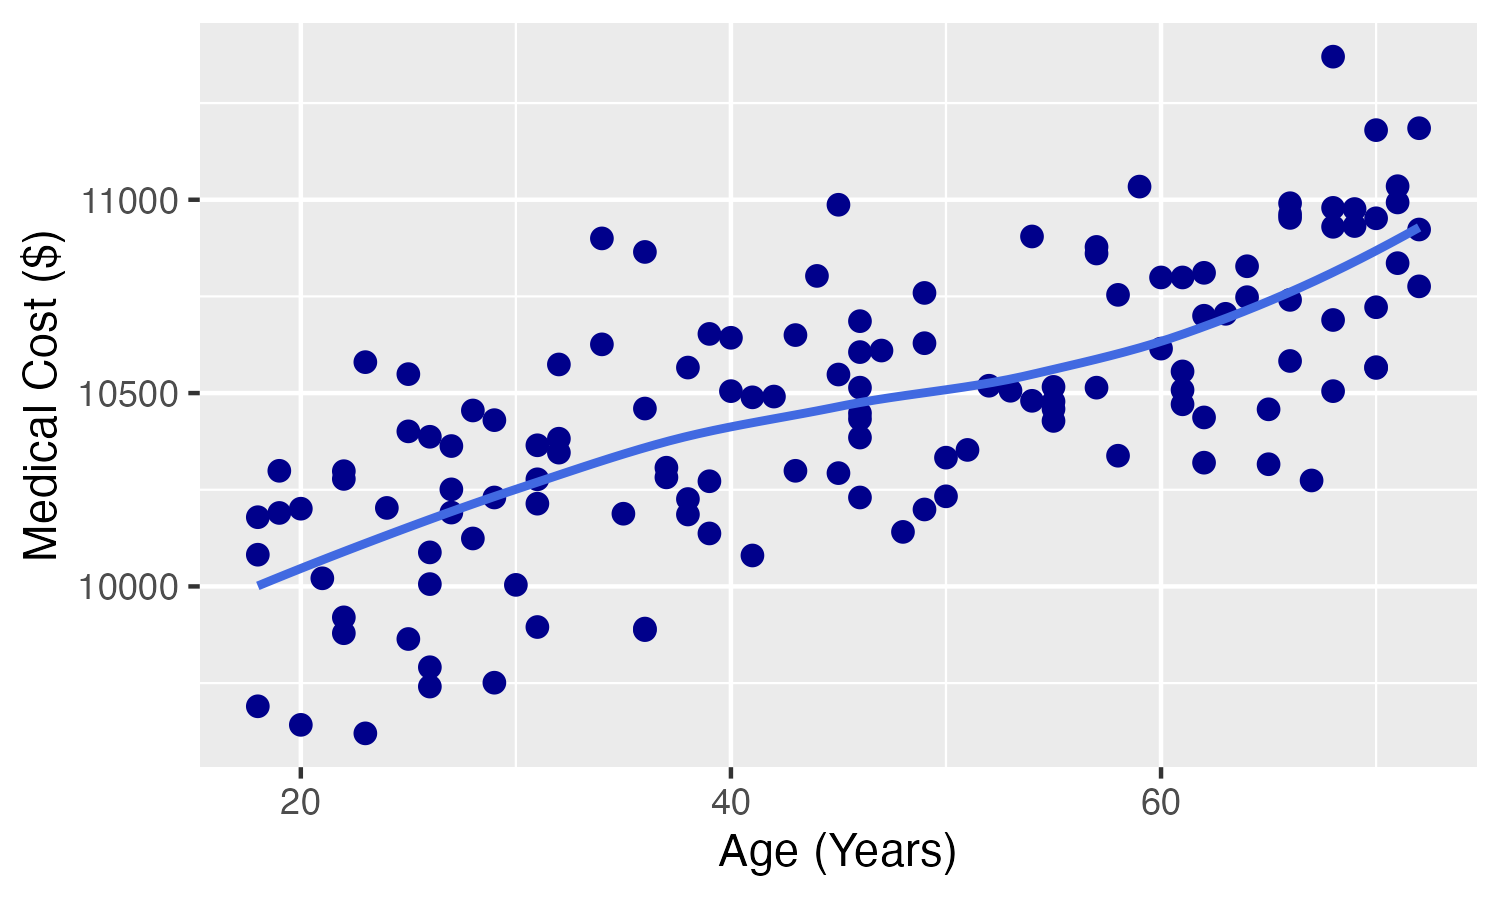
\includegraphics[keepaspectratio]{trend_plot.png}}

}

\caption{\label{fig-cost-trend}Cost Trend by Age Among Individuals with
Cardiac Events}

\end{figure}%

\textsubscript{Source:
\href{https://tracychid.github.io/EPI203_Assignment4/index.qmd.html}{Article
Notebook}}

\subsubsection{Prevalence and Odds Ratios for Cardiac
Event}\label{prevalence-and-odds-ratios-for-cardiac-event}

In this study population, the overall prevalence of a cardiac event was
5.5\% (N = 275). Of the individuals who did experience a cardiac event,
52\% (N = 142) self-reported as ever smokers and 88\% (N = 242) were
male. The average age of those who experienced a cardiac event was 47
years and the average medical cost was \$10,230 (Table 1).

\begin{table}

\caption{\label{tbl-outcomes}Multivariable logistic regression of cost
and cardiac events adjusted for sex, smoke, and age.}

\centering{

\fontsize{12.0pt}{14.0pt}\selectfont
\begin{tabular*}{\linewidth}{@{\extracolsep{\fill}}lccc}
\toprule
\textbf{Characteristic} & \textbf{OR} & \textbf{95\% CI} & \textbf{p-value} \\ 
\midrule\addlinespace[2.5pt]
Cost & 1.01 & 1.01, 1.01 & {\bfseries <0.001} \\ 
Sex &  &  & 0.3 \\ 
{\itshape     Male} & — & — &  \\ 
{\itshape     Female} & 1.35 & 0.80, 2.24 &  \\ 
Smoke &  &  & {\bfseries <0.001} \\ 
{\itshape     No Smoke} & — & — &  \\ 
{\itshape     Smoke} & 0.05 & 0.03, 0.09 &  \\ 
Age & 0.85 & 0.83, 0.87 & {\bfseries <0.001} \\ 
\bottomrule
\end{tabular*}
\begin{minipage}{\linewidth}
\vspace{.05em}
Abbreviations: CI = Confidence Interval, OR = Odds Ratio\\
\end{minipage}

}

\end{table}%

\textsubscript{Source:
\href{https://tracychid.github.io/EPI203_Assignment4/index.qmd.html}{Article
Notebook}}

In our adjusted logistic regression model, we observed a 1\% increase in
odds for a cardiac event (OR: 1.01, 95\% CI: 1.01, 1.01) for every \$1
increase in cost (Table 2). Additionally, for two key confounders, we
observed a significant finding in increased odds: individuals who
self-reported having ever smoked had 95\% lower odds of a cardiac event
compared to non-smokers and each increase in year in age was associated
with 15\% lower odds of a cardiac event. Lastly, we observed a 35\%
increase in odds for a cardiac event in females compared to males, but
the confidence interval included the null (Figure 2).

\protect\phantomsection\label{cell-fig-forest-plot}
\begin{figure}[H]

\centering{

\pandocbounded{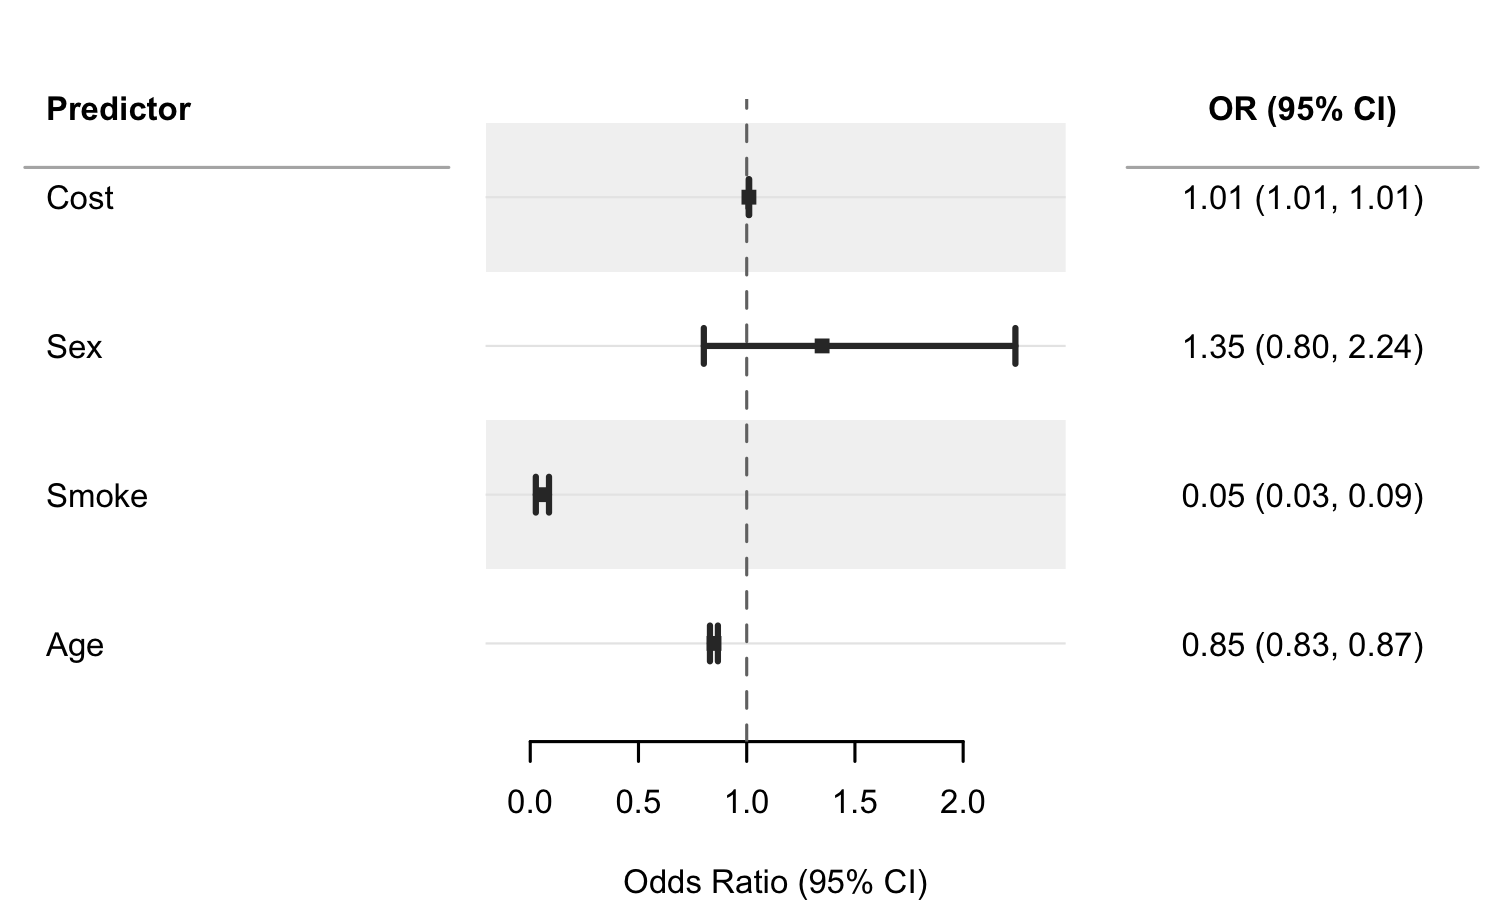
\includegraphics[keepaspectratio]{forrest_plot.png}}

}

\caption{\label{fig-forest-plot}Adjusted odds ratios of cost and cardiac
events adjusted for sex, smoke, and age.}

\end{figure}%

\textsubscript{Source:
\href{https://tracychid.github.io/EPI203_Assignment4/index.qmd.html}{Article
Notebook}}

\subsection{Discussion}\label{discussion}

In this study, we found that cost is associated with an increase in odds
for cardiac events. Biological and behavioral health factors were
associated with the relationship of interest; specifically, sex and
identifying as female were associated with increased odds in
experiencing a cardiac event and smoking was associated with lower odds
of experiencing a cardiac event. Our finding that smoking was associated
with lower odds of cardiac events is counter to current literature which
has strongly established a causal relationship in smoking increasing the
risk for cardiac events. We believe that our findings that smoking is
protective (OR = 0.05, CI = 0.03, 0.09) may be driven by the imbalance
in smoking and rates of cardiac events in females compared to males who
make up 88\% of cardiac events in our study. Additionally, the
contractual findings we observed compared to literature may also be
driven by inherent differences in our synthetic dataset compared to
real-world data from electronic health records or claims data. Moving
forward, we will seek to perform this study on electronic health records
to validate our findings in this study.

We also acknowledge that our study is not without limitations. First,
this study used synthetic data that may not accurately reflect the true
prevalence of the variables, nor characteristics of the study
population. Future studies should seek to use non-synthetic data to
validate these findings. Secondly, the prevalence of cardiac events in
this study population was rare, which may have the potential to
introduce statistical bias or generous significance levels. However,
given the ability to interpret the odds ratio as risk ratio in rare
outcomes, we pursued the use of logistic regression despite the 5.5\%
prevalence of cardiac events in our study population. Lastly, we
observed extreme class imbalance between cardiac events in men and
women, with men experiencing the majority of cardiac events.

In summary, our findings suggest an association between cost and cardiac
events controlling for biological and behavioral health factors further
adding evidence of the influence economic factors have on health,
particularly cardiovascular diseases and hospitalizations.

\subsection{Generative AI Statement}\label{generative-ai-statement}

All work, graphics/visuals, writing, study design, data analysis, and
work to produce this manuscript was completed without the use of
generative AI technology (e.g., ChatGPT).




\end{document}
